\documentclass[a4paper, 12pt]{article}
\usepackage{graphicx}
\usepackage{xcolor}
\usepackage{tikz}
\usepackage{scalerel}
\usepackage{fancyhdr}
\usepackage{tikz, pgfplots, tkz-euclide,calc}
\usepackage{geometry}
 \geometry{
        total = {160mm, 237mm},
        left = 25mm,
        right = 35mm,
        top = 30mm,
        bottom = 30mm,
      }
      
\usepackage{tabularx}
\usepackage{fancyhdr}
\usepackage{graphicx}
\usepackage{amssymb}
\usepackage{amsmath}
\usepackage{multicol}
\usepackage{graphicx}
\usepackage{wrapfig}
\usepackage{enumitem}
\usepackage{lastpage}
\usepackage{listings}
\usepackage{transparent}
\usepackage{cancel}
\usepackage{setspace}

\definecolor{pgray}{rgb}{0.5,0.5,0.5}
\definecolor{pblue}{rgb}{0.13,0.13,1}
\definecolor{pgreen}{rgb}{0,0.5,0}
\definecolor{pred}{rgb}{0.9,0,0}
\definecolor{pgrey}{rgb}{0.46,0.45,0.48}
\definecolor{pcyan}{HTML}{D4EFFC}
\definecolor{lblue}{HTML}{00AEEF}
\definecolor{input}{HTML}{AAE1FA}
\definecolor{bg}{rgb}{0.95, 0.95, 0.92}
\definecolor{vscode}{HTML}{282A36}

\onehalfspacing
\newcommand{\blue}[1]{\textcolor{blue}{#1}}
\lstdefinestyle{output}{
    language=Java,
    backgroundcolor=\color{vscode},
    basicstyle=\small\ttfamily\color{white},
    frame=single,
    escapeinside={(*}{*)},
    showspaces=false,
    showtabs=false,
    breaklines=true,
    showstringspaces=false,
    breakatwhitespace=true,
    }

\lstdefinestyle{standard}{language=Java,
    showspaces=false,
    showtabs=false,
    breaklines=true,
    showstringspaces=false,
    breakatwhitespace=true,
    commentstyle=\color{pgray},
    keywordstyle=\color{pblue},
    stringstyle=\color{pgreen},
    basicstyle=\small\ttfamily,
    frame=single,
    backgroundcolor=\color{bg},
    escapeinside={(*}{*)},}

\title{Tugas Pertemuan 2}
\author{Dhanar A \& Fajar A}
\date{17 September 2024}

\begin{document}

\maketitle

\section*{Problems}
\begin{enumerate}
    \item Buatlah sebuah program dengan input menit menjadi tahun dan hari. \\
    Hint :
    \begin{lstlisting}[style=standard]
    ....
    ....
    double minutesInYear = 60 * 24 * 365;
    ....
    \end{lstlisting}
    Gunakan Scanner , dan jelaskan step by step !\\

    \textbf{\textit{Input}} (Dalam Menit)
    \begin{enumerate}
        \item 3456789 
        \item 60 
        \item 1440 
    \end{enumerate}
    \textbf{\textit{Output}}
    \begin{enumerate}
        \item 3456789 menit  mendekati 6 tahun dan 210 hari
        \item 60 menit  mendekati 0 tahun dan 0 hari
        \item 1440 menit  mendekati 0 tahun dan 1 hari
    \end{enumerate}
    \newpage
    \item  Diberikan sebuah bangun ruang berbentuk tabung dengan setengah bola di setiap ujungnya .
    \begin{center}
        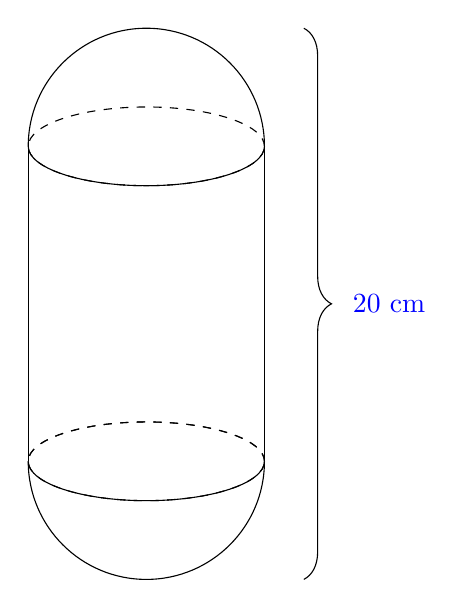
\begin{tikzpicture}
        % Draw the top ellipse
        \draw[dashed] (0,0) ellipse (1.5 and 0.5);
        
        % Draw the sides of the cylinder
        \draw (-1.5,0) -- (-1.5,-4);
        \draw (1.5,0) -- (1.5,-4);
        
        % Draw the bottom ellipse
        \draw[dashed] (0,-4) ellipse (1.5 and 0.5);
        
        % Draw the solid bottom part of the ellipse
        \draw (-1.5,-4) arc (180:360:1.5 and 0.5);
        
        % Draw the dotted top part of the ellipse
        \draw[dashed] (1.5,-4) arc (0:180:1.5 and 0.5);

        \draw (-1.5,0) arc (180:360:1.5 and 0.5);
        \draw (-1.5,0) arc (180:0:1.5 and 1.5);
        
        \draw (-1.5,-4) arc (180:360:1.5 and 1.5);

        \draw[decorate,decoration={brace,amplitude=10pt}] (2,1.5)--(2,-5.5) node[midway,right=0.5cm,blue] {$20$ cm};
        \end{tikzpicture}
    \end{center}
    
        Buatlah sebuah program untuk menghitung luas permukaan dari bangun tersebut jika diketahui diameter bangun tersebut adalah hasil dari operasi shift-right 1 bit terhadap panjangnya , kemudian jelaskan step by step !\\

        \textbf{\textit{Output :}}\\
        Luas Permukaan Total = $628$ cm$^2$    
        

    \newpage
    \item Analisis lah dan jelaskan proses Kodingan berikut ini step by step kemudian tentukan outputnya 
    \begin{lstlisting}[style=standard]
public class soal3 {
    static int a;
    static int b;
    public static void main (String[] args){
    int x = 5;
    int y = 6;
    x++;
    a = x;
    b = a;
    b = y;
    ++y;
    boolean z = a < b ? true : false;
    System.out.println(z);
    }
}
    \end{lstlisting}
\end{enumerate}
\end{document}
